\section{Ejercicio I: Algoritmo exacto}

\subsection{Introducci\'on}

Backtracking es una técnica para encontrar solución a algunos problemas computacionales, que incrementalmente construye candidatos a solución y abandona cada candidato parcial inmediatamente tras chequear que este no puede ser completado para generar una solución válida. Se utiliza en caso de que el problema admita como solución a un candidato ``parcial''.
Para esta solución pensamos a los gimnasios y paradas como nodos de un grafo completo donde los pesos de las aristas equivalen a la distancia entre los nodos.


\begin{comment}
A continuación se puede observar un psuedocódigo para la idea general de backtracking.
\begin{algorithm}[H]
\label{}
\caption{Idea general de backtracking}
\begin{algorithmic}[1]
\Statex \underline{Entrada}: S un conjunto de elementos que no forman parte de la soluci\'on parcial, N la lista de elementos de la soluci\'on parcial
\medskip
\If{solucionP(N)}
        \State nodosConsiderados $\gets$ nodos que forman el camino hallado por el algoritmo goloso
    }
    \Else
        \State nodosConsiderados $\gets$ nodos que representan a las pokeparadas del grafo
    \EndIf

\State s* $\gets$ s $\in$ S
\While{($\exists$ s $\in$ N(s*)) f(s) $<$ f(s*)}
    \State s* $\gets$ s $\in$ N(s*) tal que f(s) $<$ f(s*)
\EndWhile
\medskip
\Statex \underline{Salida}: s*
\end{algorithmic}
\end{algorithm}

procedure bt(c)
  if reject(P,c) then return
  if accept(P,c) then output(P,c)
  s ← first(P,c)
  while s ≠ Λ do
    bt(s)
    s ← next(P,s)

En el primer llamado a la función, S es el conjunto con todos los elementos que se podrían utilizar en una solución, y N es un conjunto vacío, ya que aún no se ha chequeado nada.
\end{comment}



\subsection{Algoritmo}

La solución que implementamos para obtener el camino óptimo es un backtracking. 
Para analizar cada camino utilizamos los siguientes criterios:
\begin{itemize}
    \item Si el camino que se está chequeando pasa por todos los gimnasios y recorre menos distancia que la mejor solucion encontrada hasta el momento, se reemplaza esa solución con el camino actual.
    \item Si la distancia del camino actual es mayor a la distancia del mejor encontrado, no se chequean mas caminos que partan de este.
    \item Si la distancia del camino actual es menor a la distancia del mejor hallado, y es un movimiento válido (en caso de ser un gimnasio el último nodo agregado al camino, habrá que chequear que las pociones fueran suficientes para vencerle); entonces se verifican todos los caminos que partan desde este último, sólo teniendo en cuenta como continuación los nodos que aún no están en el camino actual.
\end{itemize}

\begin{comment}
\begin{algorithm}[H]
\label{}
\caption{B\'usqueda local}
\begin{algorithmic}[1]
\Statex \underline{Entrada}: camino : \texttt{Camino} y criterio : \texttt{Vecindad}
\Statex \underline{Entrada}: S un conjunto de soluciones, N una funci\'on que devuelve las soluciones vecinas a otra dada y f una funci\'on que eval\'ua una soluci\'on
\medskip
\State camino.asignarSoluci\'onGolosa()
\If{camino.encontr\'eCamino()}
    \If{criterio == permutaCamino}
        \State nodosConsiderados $\gets$ nodos que forman el camino hallado por el algoritmo goloso
    \Else
        \State nodosConsiderados $\gets$ nodos que representan a las pokeparadas del grafo
    \EndIf
    \State busco $\gets$ true
    \State dicc(int, conj(int)) nodosCambiados $\gets$ Vac\'io()
    \While{busco}
        \While{camino.encuentroSoluci\'onVecinaMejor(nodosConsiderados)}
            \If{\#nodosCambiados.claves() $>$ 0}
                \State nodosCambiados $\gets$ Vac\'io()
            \EndIf
        \EndWhile
        \If{$\neg$camino.encuentroSoluci\'onVecinaIgual(nodosConsiderados, nodosCambiados)}
            \State busco $\gets$ false
        \EndIf
    \EndWhile
\EndIf
\medskip
\Statex \underline{Salida}: camino.imprimirSoluci\'on()
\end{algorithmic}
\end{algorithm}
\end{comment}


\subsection{Complejidad}

El backtracking, a lo sumo chequea cada combinacion posible de gimnasios y paradas en todos sus ordenes posibles; lo que, dicho de otra manera serían todas las permutaciones de cada subconjunto de partes del conjunto de nodos. 
Como cada permutacion de longitud k se construye a partir de una permutación de longitud k-1, no necesitamos construir ningún camino más de una vez.
Esto nos lleva a ver que lo que recorremos es un arbol, donde la raíz es el "conjunto vacío" (no haber recorrido nada) y el camino simple desde la misma hasta cada hoja es una permutación diferente de longitud n, donde n es la cantidad de nodos.
Habiendo entendido esto, llegamos rapidamente a la conclusión de que nuestro backtracking pertenece a la clase de complejidad \bigo{n!} ya que construye a lo sumo todas las permutaciones de longitud n, las cuales contienen a todas las de tamaños menores.


\subsection{Experimentaci\'on}

Planteamos dos experimentos diferentes para el backtracking. Para ambos utilizamos instancias en las que los gimnasios representan un tercio de los nodos, y las paradas, los nodos restantes.

El primero consiste en corroborar que la cota teórica de complejidad calculada se cumple en la práctica. Para esto utilizamos instancias del problema en las que es necesario pasar por la totalidad de las paradas para poder vencer en todos los gimnasios (acomodando adecuadamente los requerimientos de pociones). 
A continuación observamos un gráfico en el que se refleja la división entre la función obtenida a partir de medir los ticks del clock en función de la cantidad de nodos y la función de complejidad

\begin{figure}[H]
  \begin{center}
    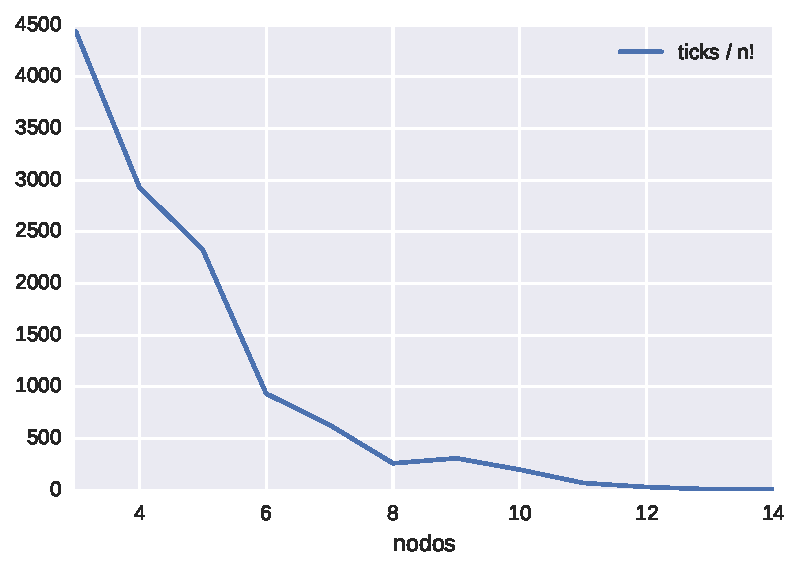
\includegraphics[scale = 0.5]{imagenes/ej1_complejidad.pdf}
    \caption{Ticks de clock / n! en función de la cantidad de nodos.}
    \label{fig:ej1_complejidad}
  \end{center}
\end{figure}

Como podemos observar en la figura \ref{fig:ej1_complejidad}, la funcion N! / cantidad de ticks es decreciente, lo que muestra que N! acota superiormente a nuestra implementación.


Para el segundo experimento, definimos un parámetro de dificultad que representa el porcentaje de paradas necesarias para poder triunfar en todos los gimnasios. Creemos que a medida que aumenta esta dificultad, el backtracking tardará más en encontrar alguna solución viable y podará menos soluciones parciales, por lo que tomará más tiempo de ejecución.
Aquí debajo podemos ver un heatmap en el que mostramos la cantidad de ticks de reloj en función de la cantidad de nodos y de la dificultad.

\begin{figure}[H]
  \begin{center}
    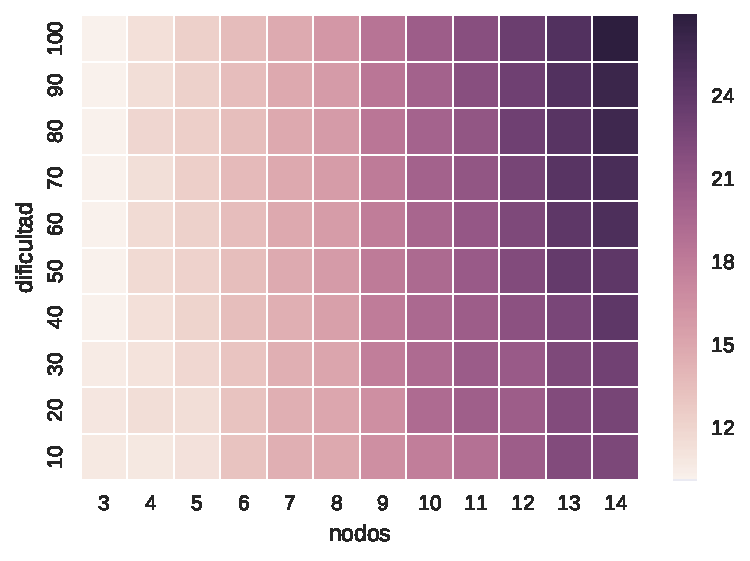
\includegraphics[scale = 0.5]{imagenes/ej1_conHeuristica.pdf}
    \caption{Ticks de clock en función de la cantidad de nodos y la dificultad.}
    \label{fig:ej1_conHeuristica}
  \end{center}
\end{figure}

Como podemos observar en la figura \ref{fig:ej1_conHeuristica}, la cantidad de ticks del clock aumenta en función de ambas variables, por lo que nuestra hipótesis está confirmada.